\documentclass{article}

% Symbols
%\usepackage{recycle}
\usepackage{amsfonts, amsthm}
\usepackage{upgreek}
\usepackage{physics}
\usepackage{cancel}
\usepackage{amssymb, latexsym, amsmath}

% Proof
\renewcommand*{\proofname}{\textbf{Demostraci\'on:}}

% Graphics
\usepackage{graphicx}
\usepackage{pgf}

% Color a letras.
%\usepackage[usenames,dvipsnames,svgnames,table]{xcolor}

% Tikz
\usepackage{tikz}
\usetikzlibrary{arrows,automata}
\usepackage{tikz}
\usetikzlibrary{arrows,automata}

\usetikzlibrary{shapes,calc}
\tikzstyle{edge}=[shorten <=2pt, shorten >=2pt,
  >=stealth, line width=1.1pt]
\tikzstyle{blueE}=[shorten <=2pt, shorten >=2pt,
  >=stealth, line width=1.5pt, blue]
\tikzstyle{blackV}=[circle, fill=black,
  minimum size=6pt,
  inner sep=0pt, outer sep=0pt]
\tikzstyle{blueV}=[circle, fill=blue, draw,
  minimum size=6pt, line width=0.75pt,
  inner sep=0pt, outer sep=0pt]
\tikzstyle{redV}=[circle, fill=red, draw,
  minimum size=6pt, line width=0.75pt,
  inner sep=0pt, outer sep=0pt]
\tikzstyle{redSV}=[semicircle, fill=red, minimum
  size=3pt, inner sep=0pt, outer sep=0pt,
  rotate=225]
\tikzstyle{blueSV}=[semicircle, fill=blue, minimum
  size=3pt, inner sep=0pt, outer sep=0pt,
  rotate=225]
\tikzstyle{blackSV}=[semicircle, fill=black, minimum
  size=3pt, inner sep=0pt, outer sep=0pt,
  rotate=225]
\tikzstyle{vertex}=[circle, draw, minimum size=6pt,
  line width=0.75pt, inner sep=0pt,
  outer sep=0pt]

% Margins
%Margins
\addtolength{\voffset}{-1cm}
\addtolength{\hoffset}{-1cm}
\addtolength{\textwidth}{2cm}
\addtolength{\textheight}{2cm}
%Header-Footer
\usepackage{fancyhdr}
\renewcommand{\headrulewidth}{1pt}

\newcommand{\set}[1]{%
  \left\{ #1 \right\}%
}

%\pagenumbering{gobble} -- Este comando
%                       -- quita el número de página.
\footskip = 50pt
\renewcommand{\headrulewidth}{1pt}

\pagestyle{fancyplain}

\begin{document}
\title{UNIVERSIDAD AUT\'ONOMA DE M\'EXICO\\ Facultad de Ciencias}
\author{Autores:
  \\ Fernanda Villaf\'an Flores
  \\ Fernando Alvarado Palacios
  \\ Adri\'an Aguilera Moreno}
\date{}
\maketitle
\begin{center}
  
\includegraphics[scale=0.20]{../Imagen/Portada.jpg}\\[0.4cm]
  \Large
  \bf{Gr\'aficas y Juegos}
  \normalsize
\end{center}
\newpage
\fancyhead[r]{ Gr\'aficas y Juegos 2022-1}
\section*{\LARGE{Tarea 3}}

\begin{enumerate}
  %%%%%%%%%%%%%%%%%%%%%%%%%%%%%%%%%%% Ejercicio 01 %%%%%%%%%%%%%%%%%%%%%%%%%%%%%%%%%%%
\item Demuestre que si $e \in E$, entonces $c(G) \le c(G-e) \le c(G) + 1$.
  
  \renewcommand\qedsymbol{QED}
  \begin{proof}
    Dado que $c$ corresponde a la función que devuelve la cantidad de componentes
    conexas, analicemos dos casos posibles:
    
    \begin{itemize}
    \item[-] Si "e" no es un puente:
      \begin{equation}
        c(G -e) = c(G)
      \end{equation}
      pues sabemos que si una arista no es puente, al borrarla, $G$ no cambia en
      número de componentes conexas y así
      \begin{equation}
        c(G) \leq c(G -e)
      \end{equation}
      pues de la dicotomia de $\leq$, cumple con la igualdad. Luego hacemos notar que
      \begin{eqnarray}
        c(G) < c(G) +1\\
        \Rightarrow c(G) \leq c(G) +1
      \end{eqnarray}
      de $1$ y $4$ se sigue
      \begin{equation}
        c(G -e) \leq c(G) +1
      \end{equation}
      de $5$ y $2$ tenemos
      \[
      c(G) \le c(G-e) \le c(G) + 1
      \]            
      
    \item[-] Si "e" es un puente:
      \begin{equation}
        c(G) < c(G -e)
      \end{equation}

      por la definición de arista como puente. Así
      \begin{equation}
        c(G) \leq c(G -e)
      \end{equation}

      pues de la dicotomia se cumple con $<$. Además sabemos que el número de
      componentes conexas aumenta exactamente en $1$ (porque estamos trabjando
      con gráficas simples) en $G -e$, de lo anterior se sigue que
      \begin{eqnarray}
        c(G -e) = c(G) +1\\
        \Rightarrow c(G -e) \leq c(G) +1
      \end{eqnarray}
      de $7$ y $9$ se sigue
      \[
      c(G) \le c(G-e) \le c(G) + 1
      \]
    \end{itemize}
    De lo anterior concluimos que $c(G) \le c(G-e) \le c(G) + 1$.
  \end{proof}
  %%%%%%%%%%%%%%%%%%%%%%%%%%%%%%%%%%% Ejercicio 02 %%%%%%%%%%%%%%%%%%%%%%%%%%%%%%%%%%%
\item Una gr\'afica es \textit{escindible completa} si su conjunto de
  v\'ertices admite una partici\'on $(S,K)$ de tal forma que $S$ es un
  conjunto independiente, $K$ es un clan, y cada v\'ertice en $S$ es adyacente
  a cada v\'ertice en $K$.   Demuestre que una gr\'afica es escindible
  completa si y s\'olo si no contiene a $C_4$ ni a $\overline{P_3}$ como
  subgr\'afica inducida.
  %%%%%%%%%%%%%%%%%%%%%%%%%%%%%%%%%%% Ejercicio 03 %%%%%%%%%%%%%%%%%%%%%%%%%%%%%%%%%%%
\item \begin{enumerate}
  %%%%%%%%%%%%%%%%%%%%% ---------- 03 (a)
\item Demuestre que si $|E| > {|V|-1 \choose 2}$, entonces $G$ es conexa.
  
  \renewcommand\qedsymbol{QED}
  \begin{proof}
    Si $|E_G| = {|V| -1 \choose 2}$, entonces hay dos posibilidades:
    \begin{itemize}
    \item[-] $G$ es conexa, entonces $G+e$ con $e \in E_G$, cumple
      \begin{eqnarray*}
        |E_{G +e}| &=& {|V| -1 \choose 2} +1\\
        &>& {|V| -1 \choose 2}
      \end{eqnarray*}
      Además $e$ no es ni lazo ni arista multiple,
      pues sabemos de resultados vistos en clase que una gráfica es completa si
      $|E| = {|V| \choose 2}$ y como
      \begin{eqnarray*}
        {|V| \choose 2} \not= {|V| -1 \choose 2}
      \end{eqnarray*}
      pues
      \begin{eqnarray*}
        {|V| \choose 2} = \frac{n \cdot (n -1)}{2}
      \end{eqnarray*}
      y
      \begin{eqnarray*}
        {|V| -1 \choose 2} = \frac{(n -1) \cdot (n -2)}{2}
      \end{eqnarray*}
      luego
      \begin{eqnarray*}
        {|V| \choose 2} &\not=& {|V| -1 \choose 2}\\
        \frac{n \cdot (n -1)}{2} &\not=& \frac{(n -1) \cdot (n -2)}{2}\\
        n \cdot (n -1) &\not=& (n -1) \cdot (n -2)\\
        n &\not=& n -2
      \end{eqnarray*}
      y de hecho
      \begin{eqnarray*}
        {|V| \choose 2} > {|V| -1 \choose 2}
      \end{eqnarray*}
      así  se justifica que $e$ no sea ni lazo, ni arista multiple. De lo anterior
      se sigue que $G +e$ es una gráfica simple que además es conexa, pues $G$ ya es
      conexa.
    \item[-] $G$ no es conexa, entonces existe un vértice aislado $x$, pues
      \begin{eqnarray*}
        {|V| -1 \choose 2} &=& \frac{|V_G|^2 -|V_G| -2 \cdot |V| +2}{2}\\
        &=& \frac{|V_G|^2 -|V_G|}{2} + \frac{2 -2|V_G|}{2}\\
        &=& \frac{|V_G| \cdot (|V_G| -1)}{2} - \frac{\cancel{2} \cdot (|V_G| -1)}{\cancel{2}}\\
        &=& {|V_G| \choose 2} - (|V_G| -1)
      \end{eqnarray*}
      y sabemos por resultados vistos en clases que hay ${|V_G| \choose 2}$ aristas en
      una gráfica completa y un vértice puede relacionarse a lo más con $|V_G| -1$ vértices
      (pues estamos trabajando con gráficas simples), nótese que de lo anterior se infiere
      que $G -x$ es conexa \footnote{pues $|E_{G -x}| = {|V_G| \choose 2}$}, así $G +e$
      (con $e \in E_G$)
      \begin{eqnarray*}
        |E_{G +e}| &=& {|V| -1 \choose 2} +1\\
        &>& {|V| -1 \choose 2}
      \end{eqnarray*}
      es conexa, pues como no hay lazos y no hay aristas múltiples en $G$, tenemos que
      la nueva arista esta comprendida entre $x$ y algún otro vértice en $V_{G -x}$ por
      lo que habrá una $xy$-trayectoria para $y \in E_G$.
    \end{itemize}
    De lo anterior concluimos que
    $|E_G| > {|V| -1 \choose 2} \Rightarrow G \text{ es conexa.}$
  \end{proof}
  %%%%%%%%%%%%%%%%%%%%% ---------- 03 (b)
\item Para $|V| > 1$ encuentre una gr\'afica inconexa con $|E| = {|V|-1
  \choose 2}$.
  
  \textbf{\textit{Solución:}}
  Si $|V_G| = 2$, como $2 > 1 \Rightarrow |V_G| > 1$, luego la
  gráfica que tiene como vértices a $u$ y $v$, y además
  \begin{eqnarray*}
    |E_G| &=& {2 -1 \choose 2}\\
    &=& \frac{(2 -1) \cdot (2 -2)}{2}\\
    &=& 0
  \end{eqnarray*}
  A continuación se muestra la gráfica mencionada:
  
  \begin{figure}[ht!]
    \centering
    \begin{tikzpicture}
      \node (0) [vertex,label=90:$u$] at (1,0){};
      \node (1) [vertex,label=90:$v$]  at (6,0){};
      
      \node (L) at (-0.5,1){$G_1$};
    \end{tikzpicture}
  \end{figure}
  Así observemos que la gráfica anterior es inconexa.
  \hfill $\square$
\end{enumerate}
  %%%%%%%%%%%%%%%%%%%%%%%%%%%%%%%%%%% Ejercicio 04 %%%%%%%%%%%%%%%%%%%%%%%%%%%%%%%%%%%
\item \begin{enumerate}
  %%%%%%%%%%%%%%%%%%%% ----------- 04 (a)
\item Demuestre que si $\delta > \lfloor \frac{|V|}{2} \rfloor - 1$,
  entonces $G$ es conexa.
  
  \renewcommand\qedsymbol{QED}
  \begin{proof}
    Para este inciso procedemos por inducción sobre $V_G$. Sea $G$ una gráfica
    con $|V_G| = 1$, así $\delta = \lfloor \frac{1}{2} \rfloor = 0$, \textit{i.e.}

    \begin{figure}[ht!]
    \centering
    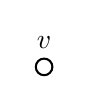
\begin{tikzpicture}
      \node (0) [vertex,label=90:$v$]  at (0,0){};
    \end{tikzpicture}
    \end{figure}
        
    donde $E_G = \varnothing$. Luego supongamos como hipótesis inductiva
    que para una cantidad $n$ de vértices, el que se cumpla $\delta = \lfloor
    \frac{|V|}{2} \rfloor$ implica que $G$ es conexa. A continuación veamos
    que pasa con $G + x$, con $x \in V_{G +x}$, así $G$ cumple con $\delta
    = \lfloor \frac{|V|}{2} \rfloor$, de lo anterior se sigue que $x$ es vecino
    de al menos $\lfloor \frac{|V|}{2} \rfloor$ vértices en $G$ (notar que $G$ es,
    de hecho, una subgráfica inducida por vértices de $G +x$), como $G$ era
    conexa por hipótesis inductiva se sigue que $G +x$ es conexa.    
  \end{proof}
  %%%%%%%%%%%%%%%%%%%% ----------- 04 (b)
\item Para $|V|$ par encuentre una gr\'afica $(\lfloor \frac{|V|}{2}
  \rfloor -1)$-regular e inconexa.
  
  \textbf{\textit{Solución:}}
  Con $|V| = 4$ tenemos
  \begin{eqnarray*}
    \lfloor \frac{4}{2} \rfloor -1 &=& 2 -1\\
    &=& 1
  \end{eqnarray*}
  
  \begin{figure}[ht!]
    \centering
    \begin{tikzpicture}
      \node (0) [vertex,label=90:$a$]  at (1,0){};
      \node (1) [vertex,label=90:$b$]  at (6,0){};
      \node (2) [vertex,label=90:$a$]  at (1,-2){};
      \node (3) [vertex,label=90:$b$]  at (6,-2){};
      
      \node (L) at (-0.5,1){$G$};
      
      \draw [edge] (0) to (1);
      \draw [edge] (2) to (3);
    \end{tikzpicture}
  \end{figure}
  
  Así la gráfica es $1$-regular e inconexa.
  \hfill $\square$
\end{enumerate}
  %%%%%%%%%%%%%%%%%%%%%%%%%%%%%%%%%%% Ejercicio 05 %%%%%%%%%%%%%%%%%%%%%%%%%%%%%%%%%%%
\item Demuestre que si $D$ no tiene lazos y $\delta^+ \ge 1$, entonces $D$
  contiene un ciclo dirigido de longitud al menos $\delta^+ + 1$.
  
  \renewcommand\qedsymbol{QED}
  \begin{proof}
    Para este ejercicio procedamos por inducción en $V$, así cuando
    $\delta^+ = 1$ y $|V| = 2$, tendremos
    
    \begin{center}
      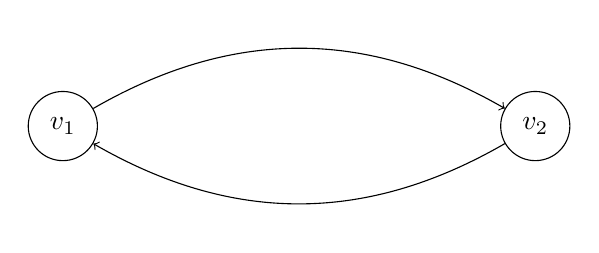
\begin{tikzpicture}[->, node distance = 3cm, auto]
        
        \node[state](v1)at(1,  0)  {$v_1$};
        \node[state](v2)at(7,  0)  {$v_2$};   
        
        %%----------------------------------
        \path (v1)edge[bend left]node{}(v2)
        (v2)edge[bend left]node{}(v1);
        %%----------------------------------
      \end{tikzpicture}
    \end{center}

    Ahora supongamos que hay un ciclo $C$ de al menos longitud $\delta^+ +1$,
    con $\delta^+ > 1$, para $n(n > 1)$ vértices en $D$ y además $D$ no
    tiene lazos. Luego para $|V_D| = n +1$, donde llamaremos $x$ al vértice
    extra, analicemos dos casos extremos:
    
    \begin{itemize}
    \item[-] Si $x$ tiene una sóla incidencia, entonces $\delta^+ = 1$ y como
      $\mathcal{L}(C) > 1$, tenemos que existe un ciclo de al menos $\delta^+ +1$
      y en este caso es estrictamente mayor. De lo anterior terminamos.
      
    \item[-] Si para cada vértice $u_i(1 < i \geq |V_D| -1)$ en $G$ hay
      una arista que "salga" de $u_i$ e incida en $x$, tenemos que $\delta^+$
      no se modifica. Ahora notemos que en partícular hay al menos
      $u_i, u_{i +1}$ tales que existe una $u_i u_{i +1}$-trayectoria en $C$
      (notar que $u_i$ y $u_{i +1}$ son vecinos), luego como existe $e_1 = u_i x$
      y $e_{2} = u_{i +1} x$, con $e_1$ y $e_2$ en $E_D$, entonces tenemos
      un nuevo ciclo que es de al menos $\mathcal{L}(C) +1$ de longitud, así
      como $\mathcal{L}(C) \geq \delta^+ +1$, tenemos que el nuevo ciclo es
      de al menos longitud $\delta^+ +1$.
    \end{itemize}
    Del análisis anterior concluimos que el enunciado se cumple.
  \end{proof}
\end{enumerate}

\section*{Puntos Extra}
\begin{enumerate}
  %%%%%%%%%%%%%%%%%%%%%%%%%%%%%%%%%%% 01 EXTRA %%%%%%%%%%%%%%%%%%%%%%%%%%%%%%%%%%%
\item Demuestre que el n\'umero de $v_i v_j$-caminos de longitud $k$ en $G$ es
  $(A^k)_{ij}$ donde $A$ es la matriz de adyacencia de $G$.
  %%%%%%%%%%%%%%%%%%%%%%%%%%%%%%%%%%% 01 EXTRA %%%%%%%%%%%%%%%%%%%%%%%%%%%%%%%%%%%
\item Sea $G$ una gr\'afica bipartita de grado m\'aximo $k$.   Demuestre que
  existe una gr\'afica bipartita $k$-regular, $H$, que contiene a $G$ como
  subgr\'afica inducida.
\end{enumerate}

\end{document}
